\section{問題設定}\label{ux554fux984cux8a2dux5b9a}

\subsection{設計目的}\label{ux8a2dux8a08ux76eeux7684}

食品工場では同時に大量の材料を撹拌する必要があるので,ロボットがあると業務効率化が図れる.さらに,食品材料の撹拌という工程では,低速で混ぜた場合に「ダマ」と呼ばれる呼ばれる固形物ができてしまう事があるため,ロボットの手先速度を上げる必要がある.目標となる手先速度及び加速時間の2つから必要となる手先加速度を計算し,その手先角速度が必要条件を満たすように設計する.

\subsection{食品撹拌ロボットの製品目標値・設計仕様}\label{ux98dfux54c1ux64b9ux62ccux30edux30dcux30c3ux30c8ux306eux88fdux54c1ux76eeux6a19ux5024ux8a2dux8a08ux4ed5ux69d8}

今回作成する食品撹拌ロボットの製品目標値・設計仕様を表\ref{first-spec}に示す.表\ref{first-spec}で決めた評価基準を満たすよう設計を行う.

\begin{table}[htb]
\caption[]{食品撹拌ロボットの製品目標値・設計仕様}
  \begin{center}
    \begin{tabular}{|c|c|} \hline
      製品名 & 食品撹拌ロボット \\ \hline \hline
      関節駆動トルク [Nm] & 393.0 \\ \hline
      回転軸からアーム中心部のブレードまでの長さ [m] & 1.0  \\ \hline
      回転軸からアーム先端部のブレードまでの長さ [m] & 1.0  \\ \hline
      アーム部分総質量[kg] & 250.0  \\ \hline
      アーム部分慣性モーメント [$\rm kgm^2$] & 250 \\ \hline
      1秒あたりの回転数 [回転] & 1.0  \\ \hline
      手先加速度[$\rm m/s^2$] & 6.28 \\ \hline
      加速時間[s] & 2.0以内 \\ \hline
      許容最大たわみ(z軸方向) [mm]& $2.50$以下 \\ \hline
      安全率 & 3.0以上 \\ \hline
    \end{tabular}
    \label{first-spec}
  \end{center}
\end{table}

関節駆動トルク及び回転軸から各ブレードまでの長さを固定した.
関節駆動トルクである393.0{[}Nm{]}というのは,今回モータとして豊興工業の内接式歯車モーターである「TCM5-F125-M1-A」を使用するため,そのモータのトルクを元にして関節駆動トルクを決めた.

今回,1秒あたりの回転数を1回転と決めた.つまり,このロボットに要求される角速度は,6.28{[}rad/s{]}となる.
このロボットの加速時間は2.0{[}s{]}と決めたので,1秒以内に秒以内に要求角速度にもっていくためには角速度は3.14{[}\(\rm rad/s^2\){]}以上,つまり手先加速度が6.28{[}\(\rm m/s^2\){]}以上になるようにロボットを設計する必要がある.
上記で設定した許容最大たわみ,手先加速度,加速時間及び安全率の4つが仕様を満たすようにアームの断面形状を変更する.

\subsection{ロボットの設計}\label{ux30edux30dcux30c3ux30c8ux306eux8a2dux8a08}

今回のロボットの設計においては,軽量かつ十分な強度をもつ材料を選ぶ必要があるので,今回はアルミニウム1060を使用することとした.

今回設計したロボットの土台部分,そして軸部分の各寸法をそれぞれ図\ref{default-base},図\ref{default-shaft}に示す.

\begin{figure}[htbp]
  \begin{center}
    \begin{tabular}{c}
          \begin{minipage}{0.50\hsize}
        \begin{center}
        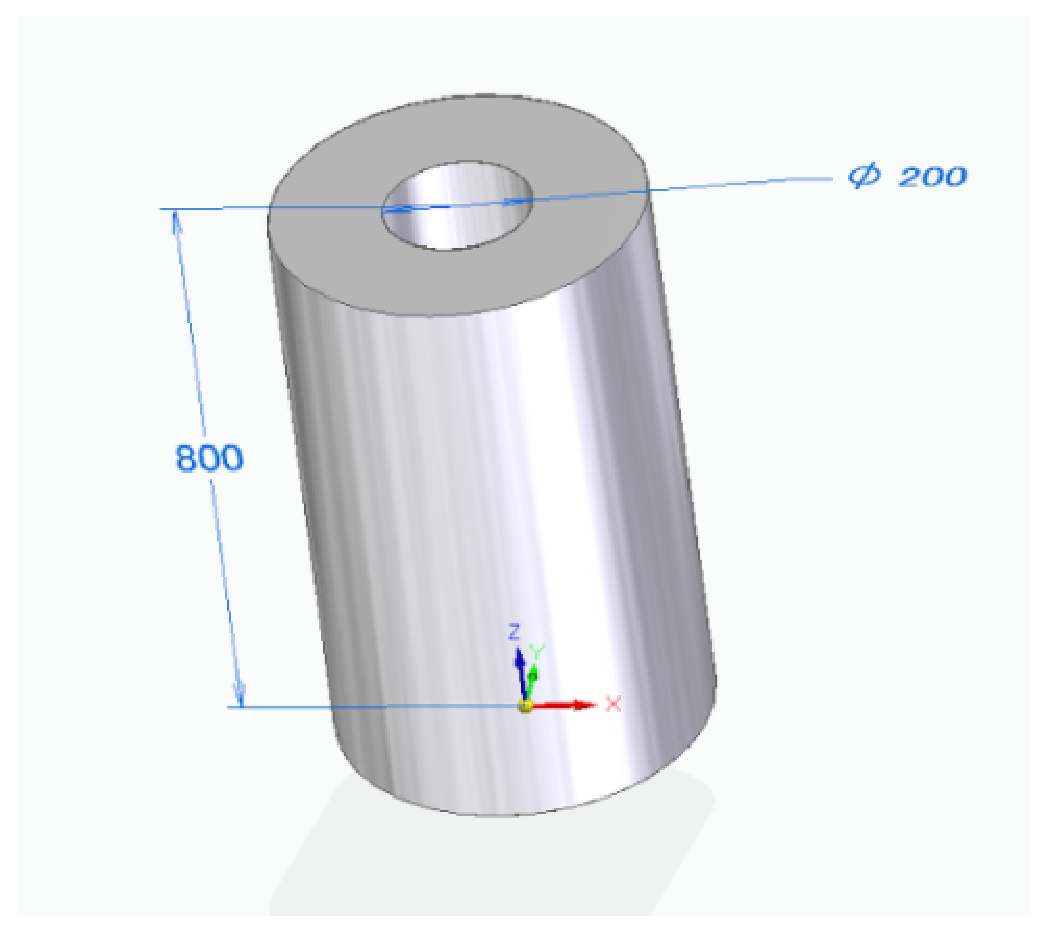
\includegraphics[height=5.5cm]{img/eps/default-base.eps}
        \caption{設計した土台の形状}
        \label{default-base}
        \end{center}
      \end{minipage}
      \begin{minipage}{0.50\hsize}
        \begin{center}
          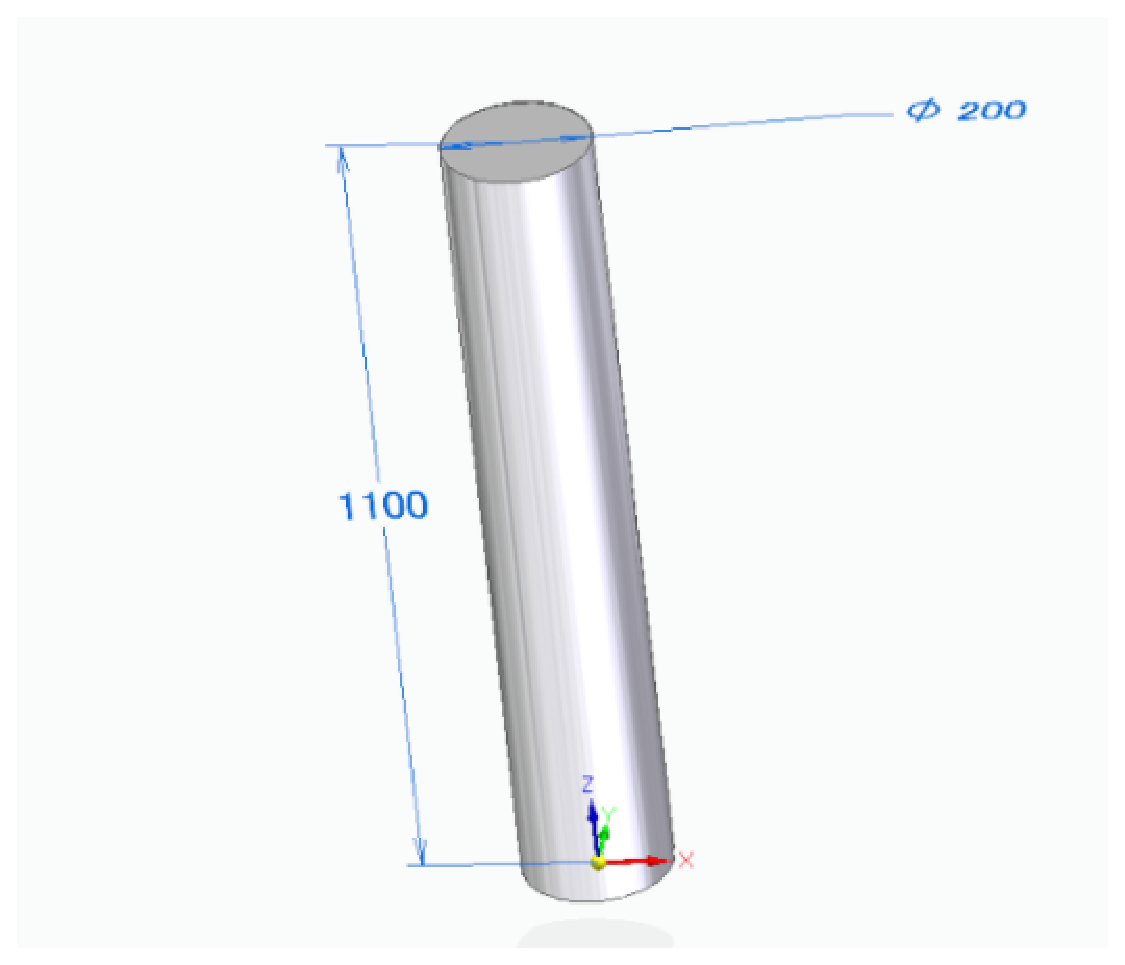
\includegraphics[height=5.5cm]{img/eps/default-shaft.eps}
          \caption{設計した軸の形状}
          \label{default-shaft}
        \end{center}
      \end{minipage}
    \end{tabular}
  \end{center}
\end{figure}

そして,今回設計したアーム部分を図\ref{default-robot-arm}に示す.アームには,撹拌のためのブレードを設置するための穴を2つあけた.

\begin{figure}[htbp]
  \begin{center}
    \begin{tabular}{c}
      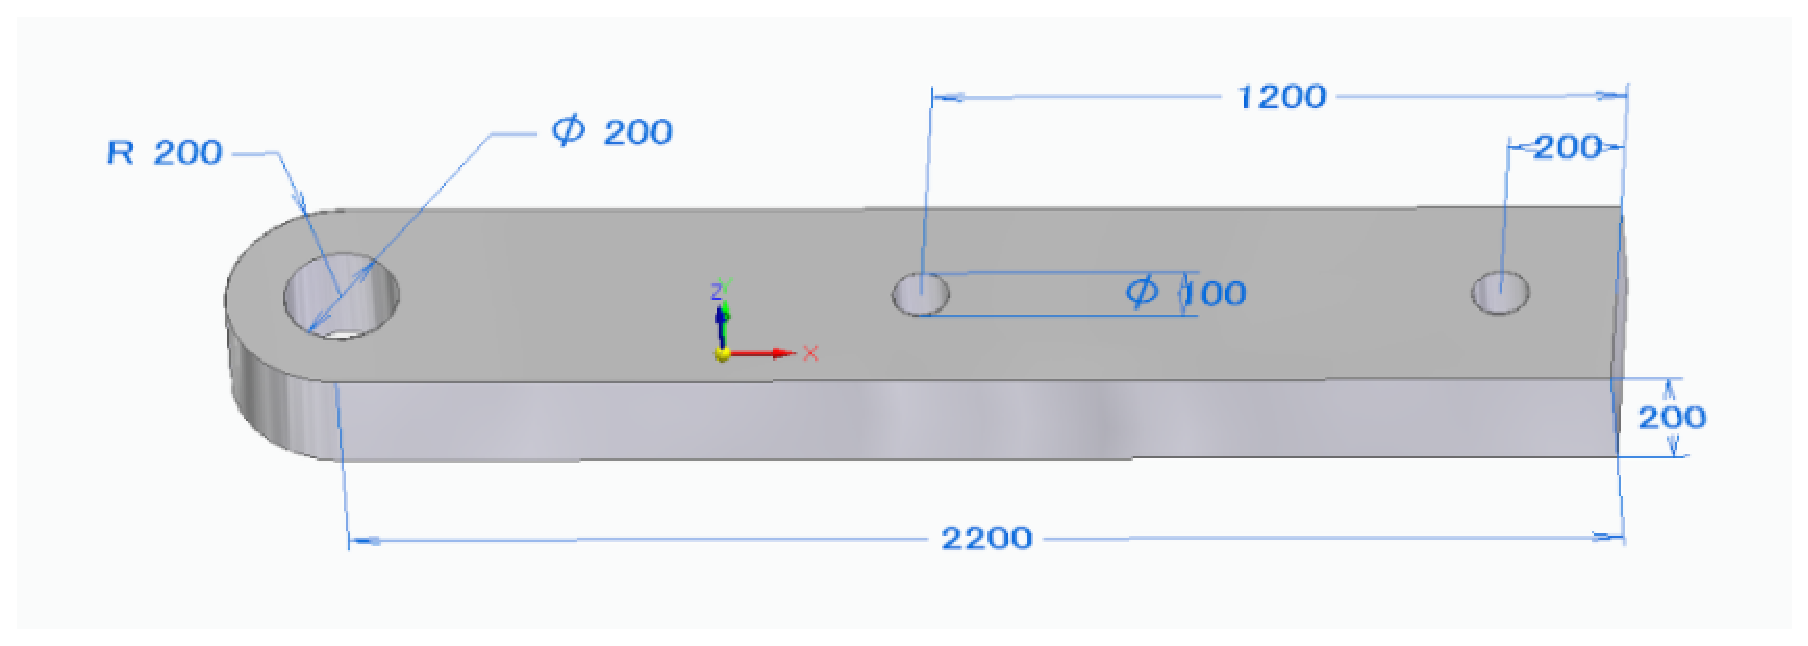
\includegraphics[height=5.0cm]{img/eps/default-robot-arm.eps}
    \end{tabular}
    \caption{設計したアームの形状}
    \label{default-robot-arm}
  \end{center}
\end{figure}

今回は中心部および先端部にミキサーのブレード部分を想定した12{[}kg{]}のおもりを付けることとした.その重りのモデルを図\ref{brade}に示す.
さらに,設計した土台,軸,及びアームをアセンブリし中心部及び先端部にブレードを取り付けたものが,図\ref{robot-arm}である.このロボットを基準ロボットとし,手先加速度や強度を考慮して再設計を行っていく.

\begin{figure}[htbp]
  \begin{center}
    \begin{tabular}{c}
          \begin{minipage}{0.30\hsize}
        \begin{center}
        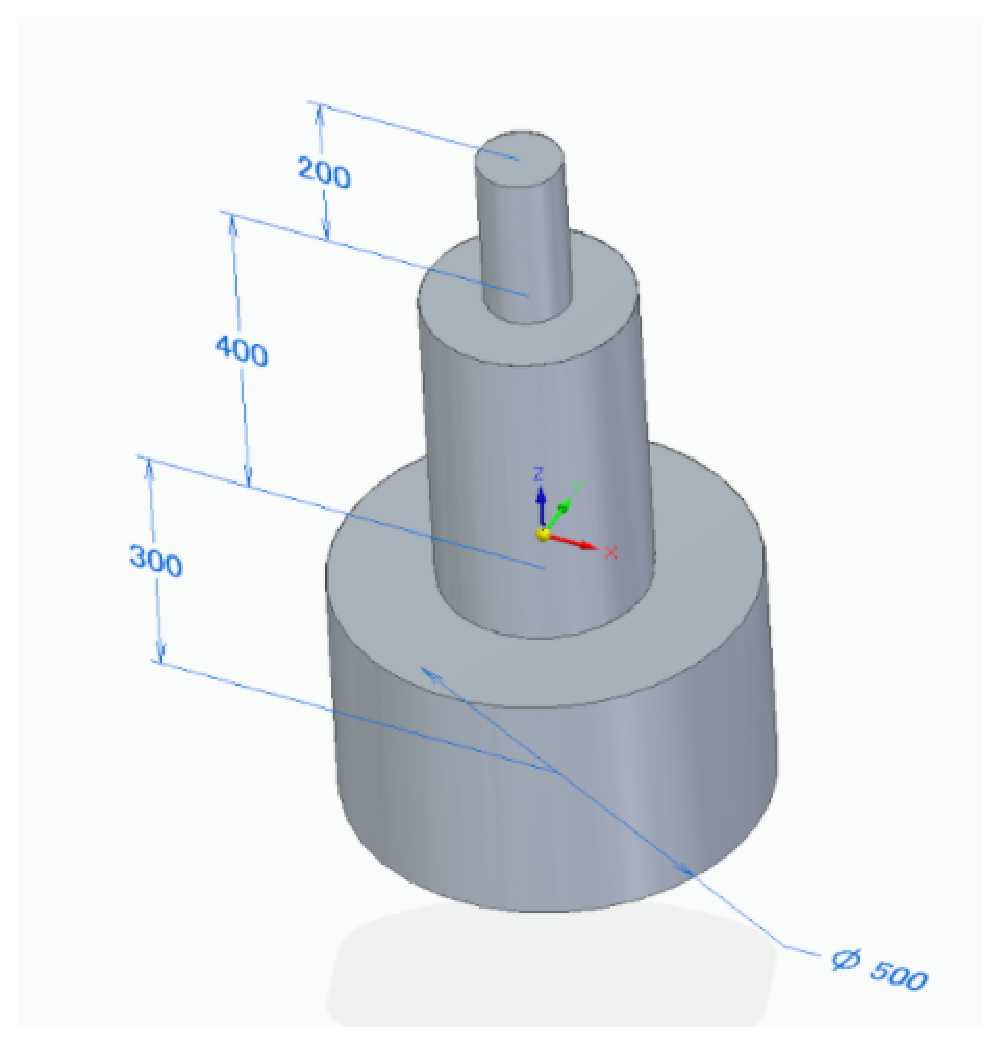
\includegraphics[height=5.5cm]{img/eps/brade.eps}
        \caption{ミキサーのブレード}
        \label{brade}
        \end{center}
      \end{minipage}
      \begin{minipage}{0.70\hsize}
      \begin{center}
        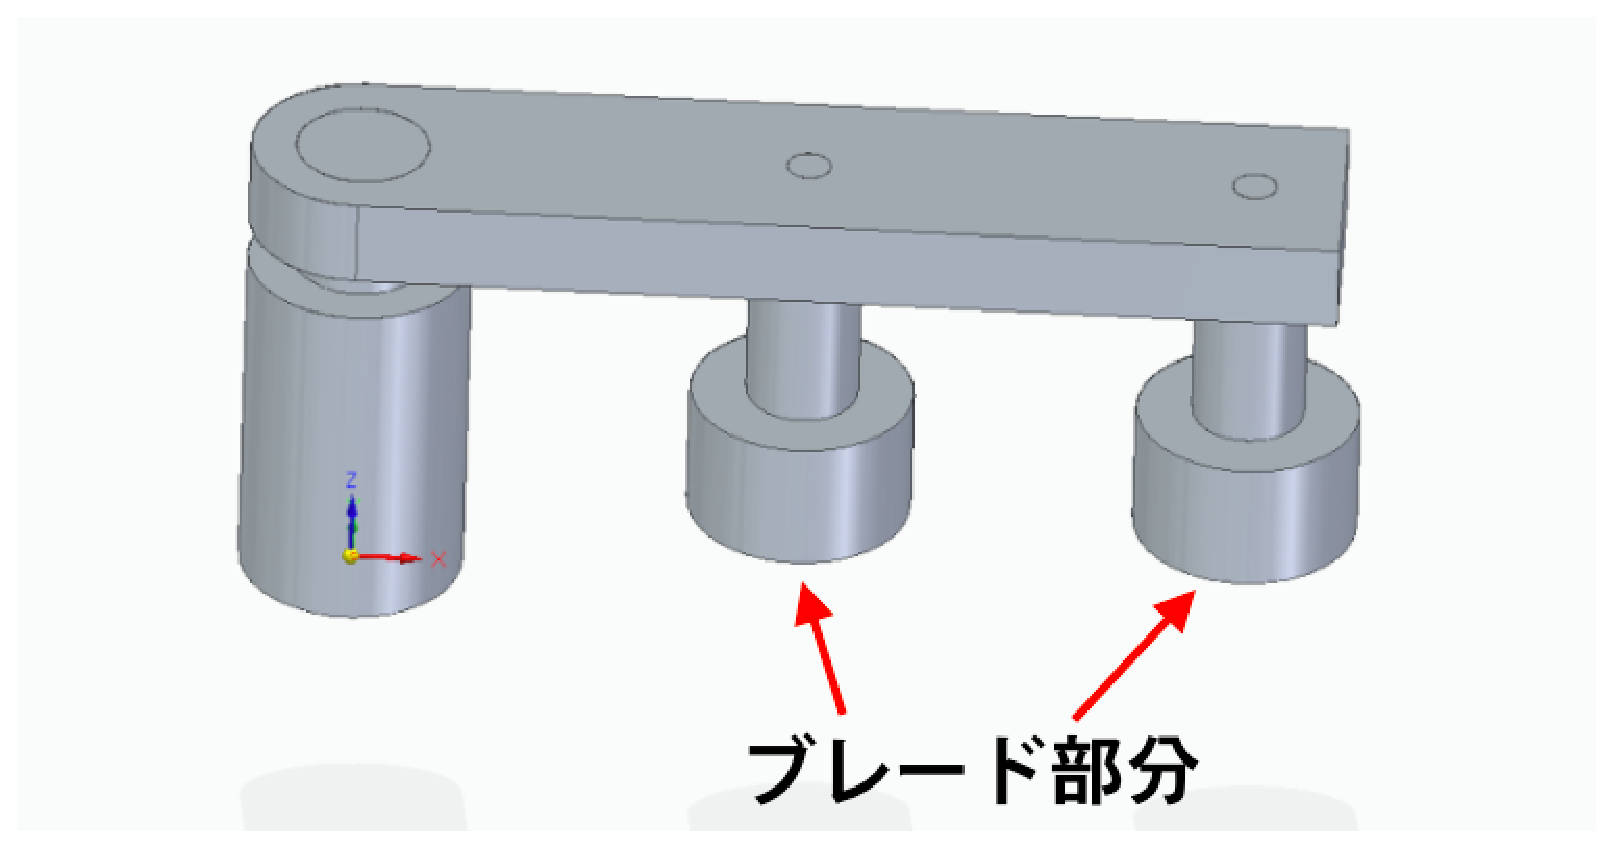
\includegraphics[height=5.5cm]{img/eps/robot-model.eps}
        \caption{基準ロボットの概形}
        \label{robot-arm}
        \end{center}
      \end{minipage}
    \end{tabular}
  \end{center}
\end{figure}

工場での作業を想定しているため,撹拌に使用する食品容器は大きく,図\ref{container-model}のような容器になっている.この容器は最大9000{[}L{]}の液状の食品が入るようになっている.

\begin{figure}[htbp]
  \begin{center}
    \begin{tabular}{c}
      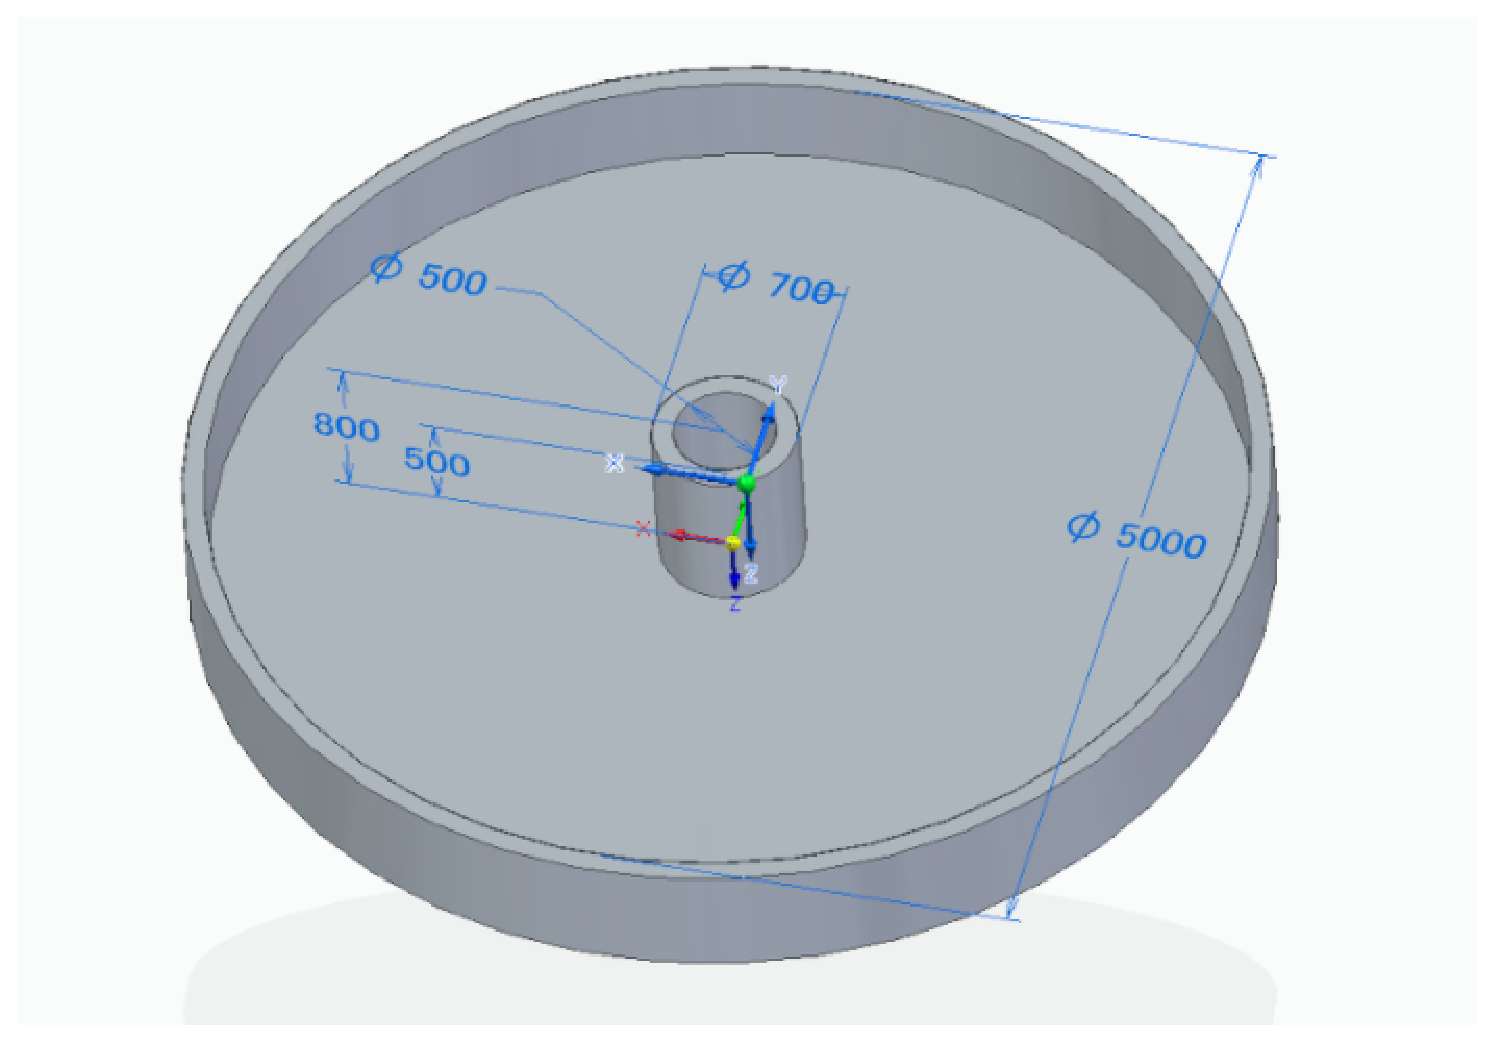
\includegraphics[height=6.0cm]{img/eps/container-model.eps}
    \end{tabular}
    \caption{食品材料を入れる容器}
    \label{container-model}
  \end{center}
\end{figure}

図\ref{container-with-robot}が,図\ref{container-model}で示した容器に図\ref{robot-arm}のロボットを設置した様子である.このようにロボットを食品が入っている容器の中心に設置し,アームを回転させることによって食品を撹拌することが出来るというわけである.

\begin{figure}[htbp]
  \begin{center}
    \begin{tabular}{c}
      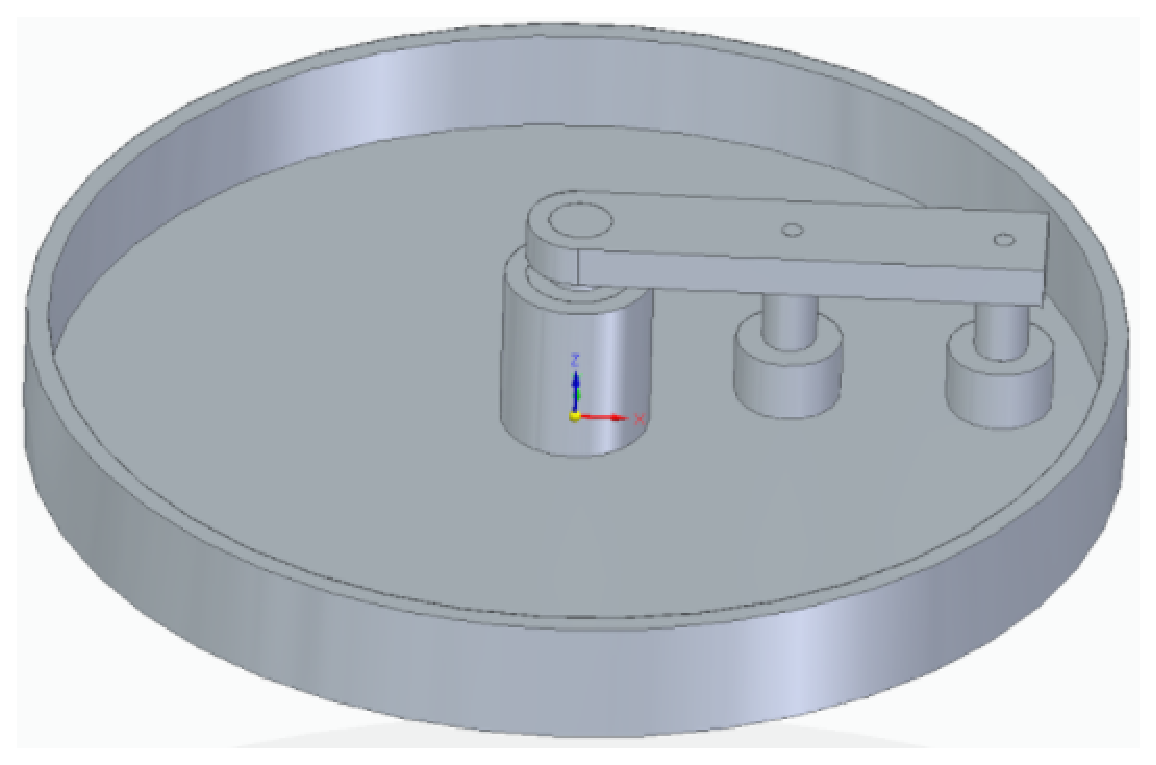
\includegraphics[height=5.5cm]{img/eps/default.eps}
    \end{tabular}
    \caption{容器にロボットを設置した様子}
    \label{container-with-robot}
  \end{center}
\end{figure}

図\ref{robot-arm}に示した基準ロボットを元に,再設計を行った.再設計を行う際には土台と軸,及びブレードを想定した12{[}kg{]}の重りは同じものを使い,アーム部分のみ再設計を行った.

手先加速度を上げるための軽量化を行ったのが図\ref{light-arm-model}に示すアームである.また,解析により,アーム先端部に比べてアーム中心部に大きい応力がかかることが分かった.その応力により生じるたわみを少なくするために中心部を太く設計したものが図\ref{strong-arm-model}のアームである.

\begin{figure}[htbp]
  \begin{center}
    \begin{tabular}{c}
          \begin{minipage}{0.45\hsize}
        \begin{center}
        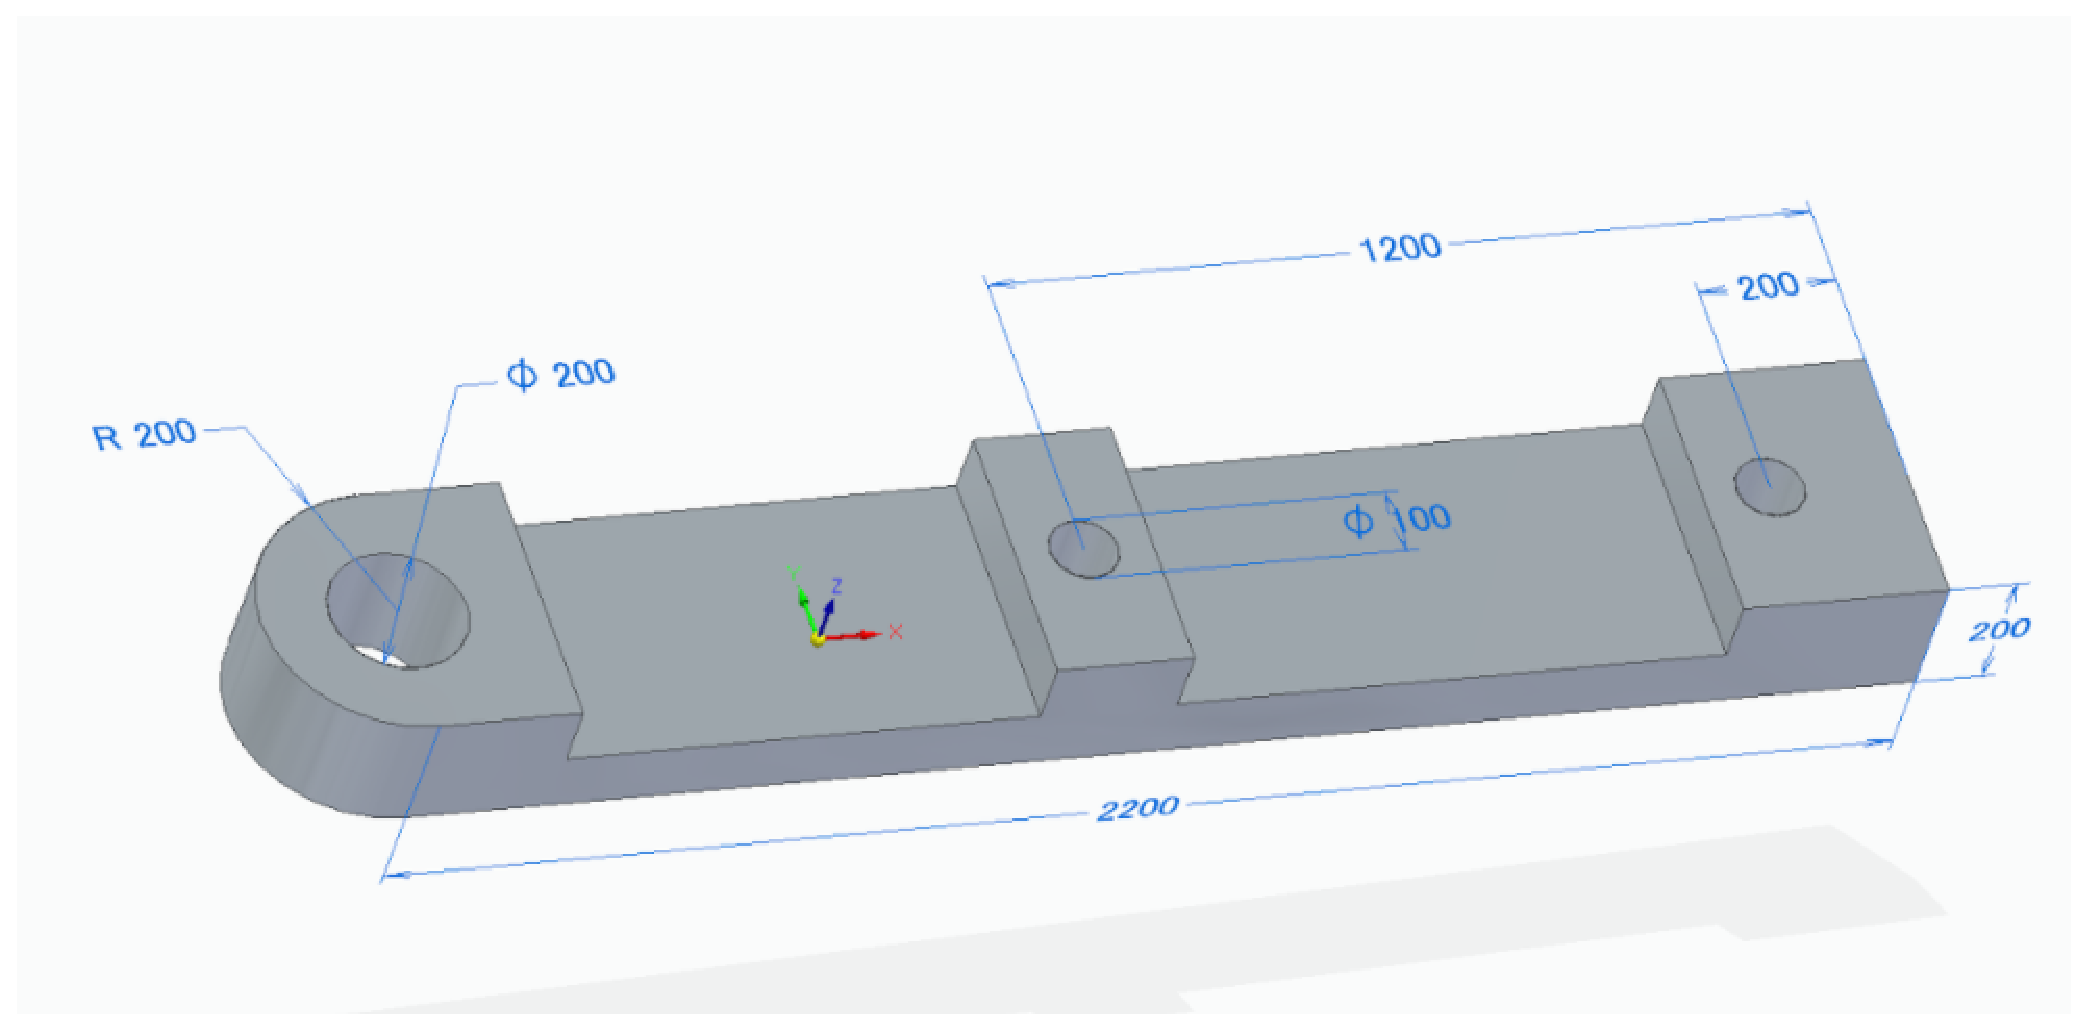
\includegraphics[height=4.0cm]{img/eps/light-arm-model.eps}
        \caption{手先加速度をあげるために再設計したアーム}
        \label{light-arm-model}
        \end{center}
      \end{minipage}
      \begin{minipage}{0.55\hsize}
        \begin{center}
          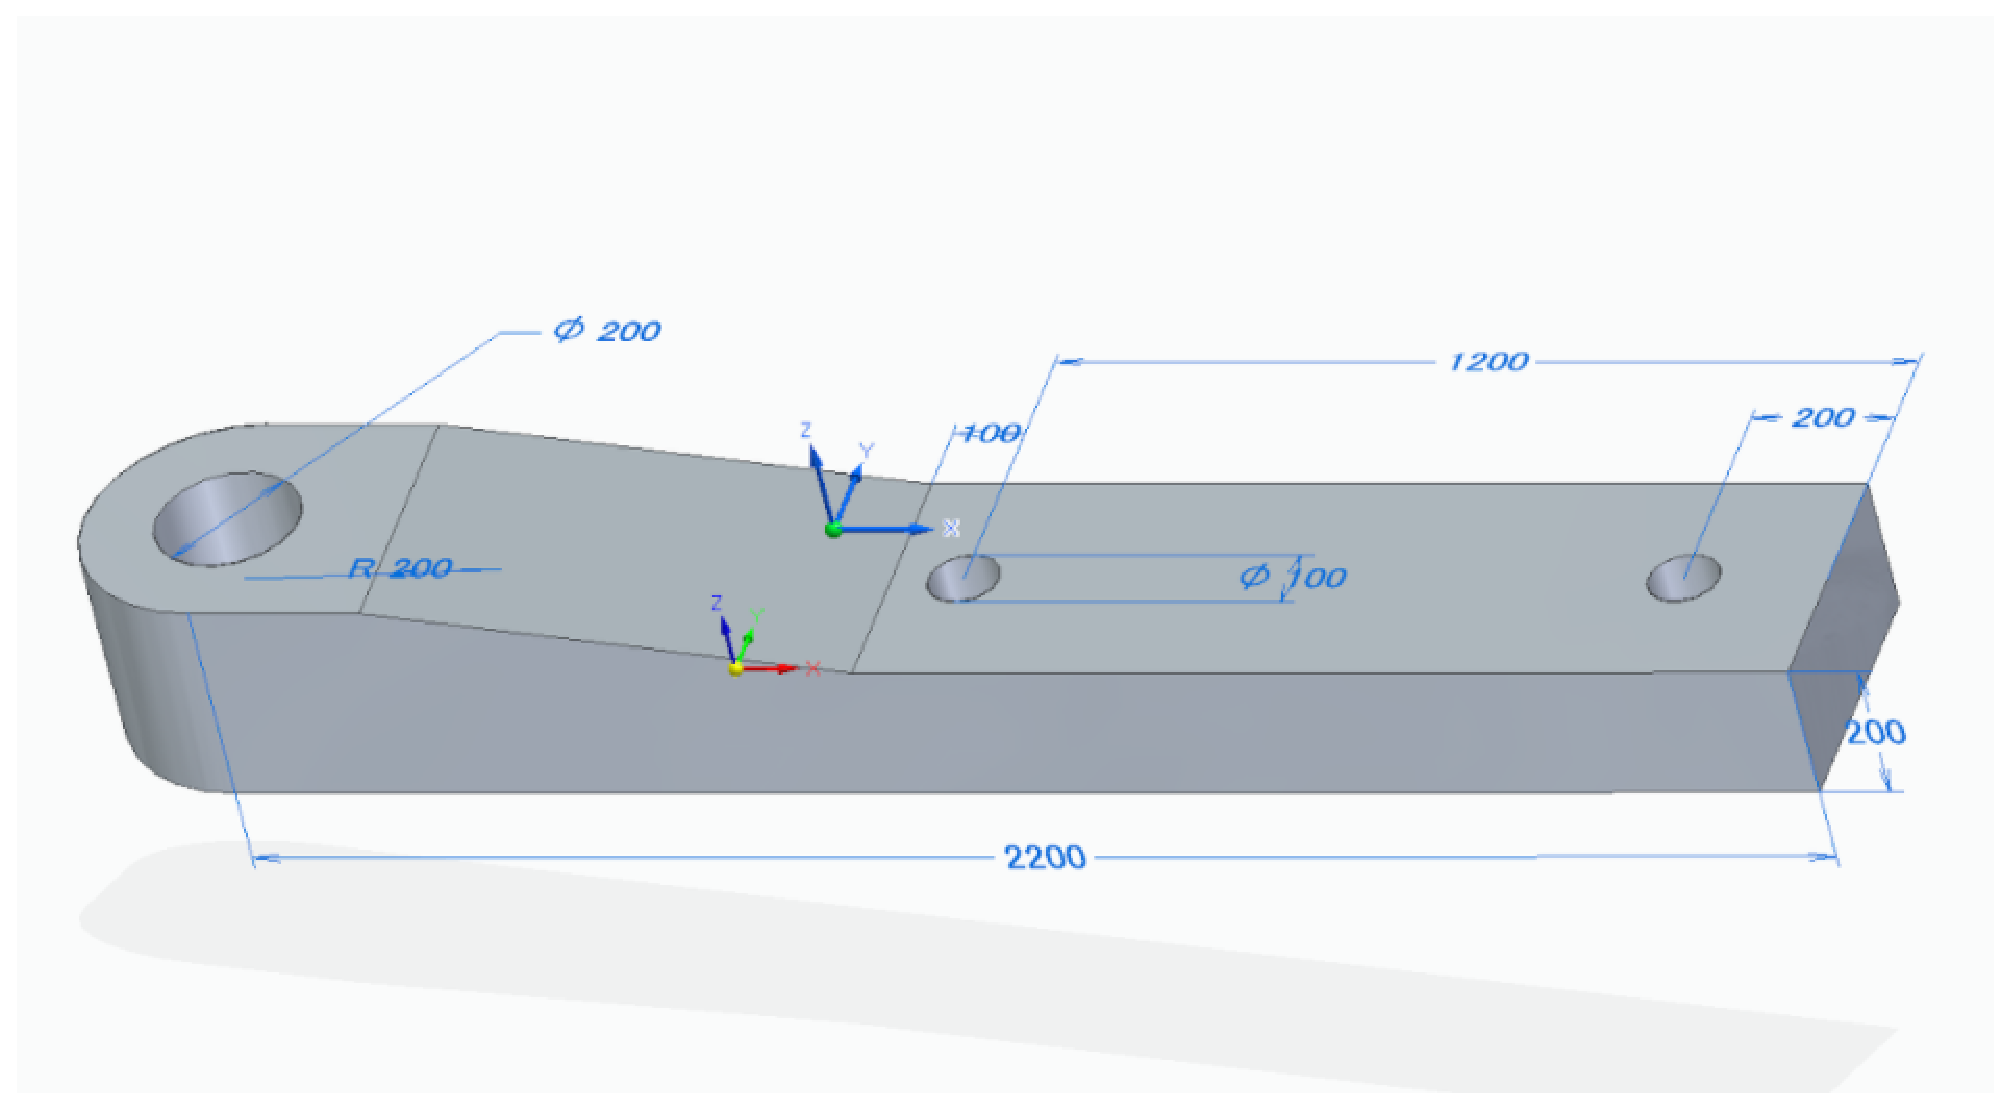
\includegraphics[height=4.0cm]{img/eps/strong-arm-model.eps}
          \caption{強度を考慮して再設計したアーム}
          \label{strong-arm-model}
        \end{center}
      \end{minipage}
    \end{tabular}
  \end{center}
\end{figure}

今回設計した3種類の形状の異なるアームをアセンブリした結果を図\label{3-arm}に示す.

\begin{figure}[htbp]
  \begin{center}
    \begin{tabular}{c}
          \begin{minipage}{0.32\hsize}
        \begin{center}
          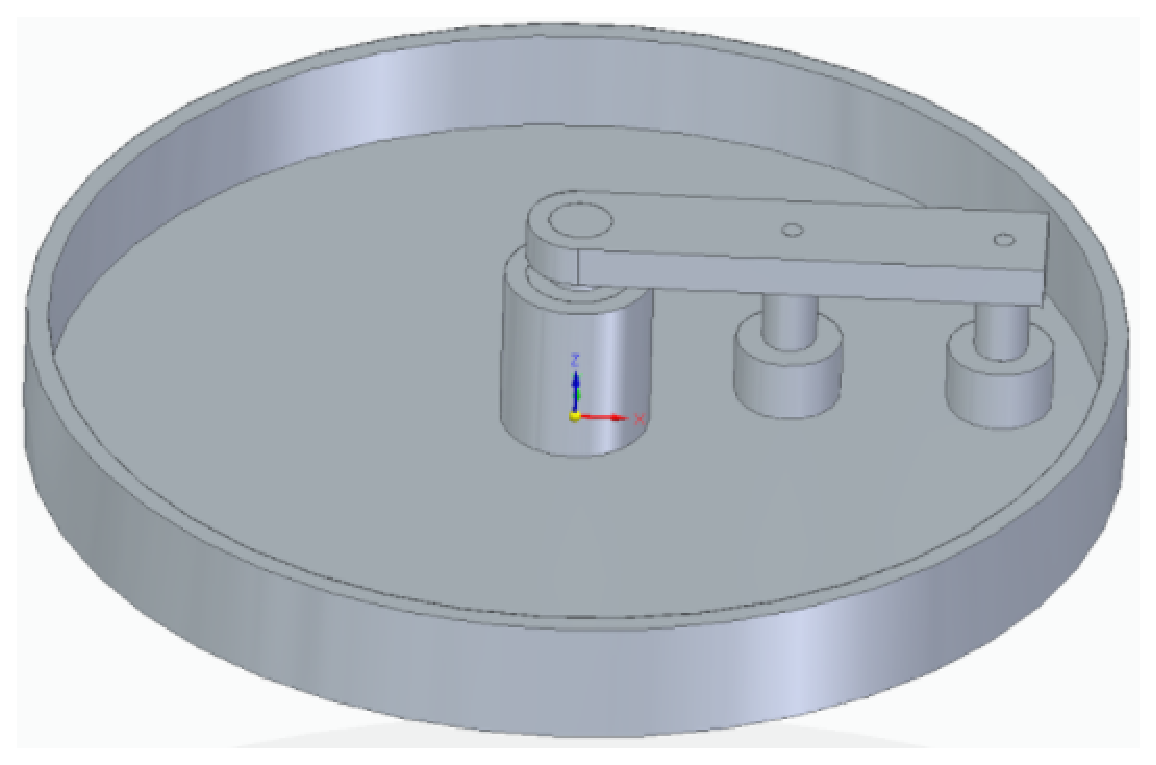
\includegraphics[height=3.1cm]{img/eps/default.eps}
          \scalebox{0.8}{[1]基準となる設計}
        \end{center}
      \end{minipage}
      \begin{minipage}{0.32\hsize}
        \begin{center}
          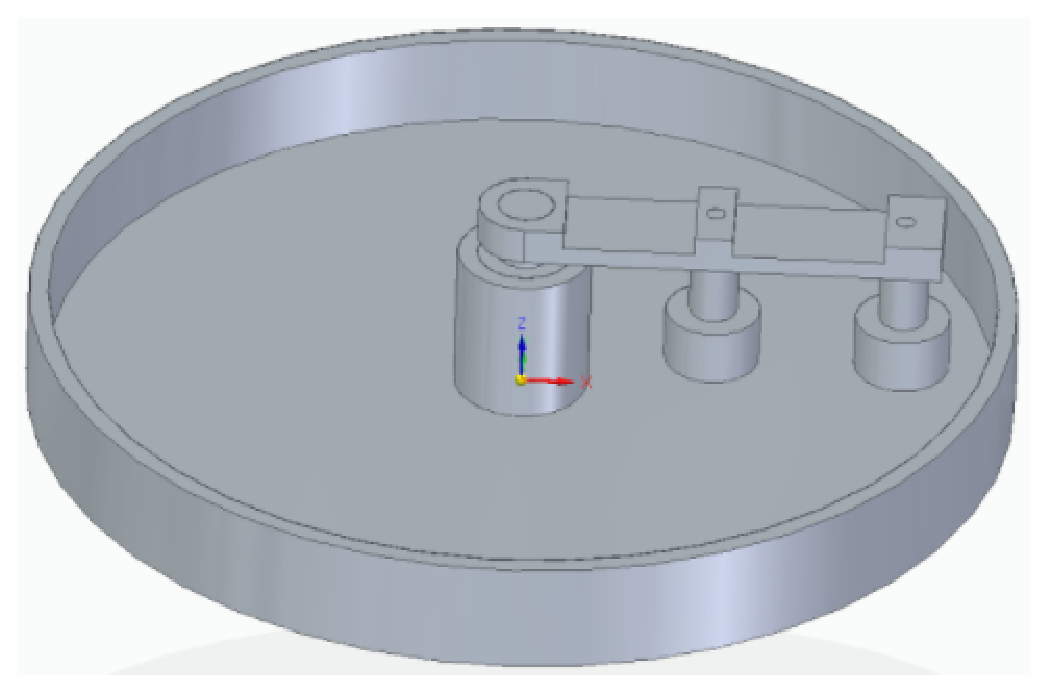
\includegraphics[height=3.1cm]{img/eps/acculate.eps}
          \scalebox{0.8}{[2]手先加速度をあげる設計}
        \end{center}
      \end{minipage}
      \begin{minipage}{0.32\hsize}
        \begin{center}
          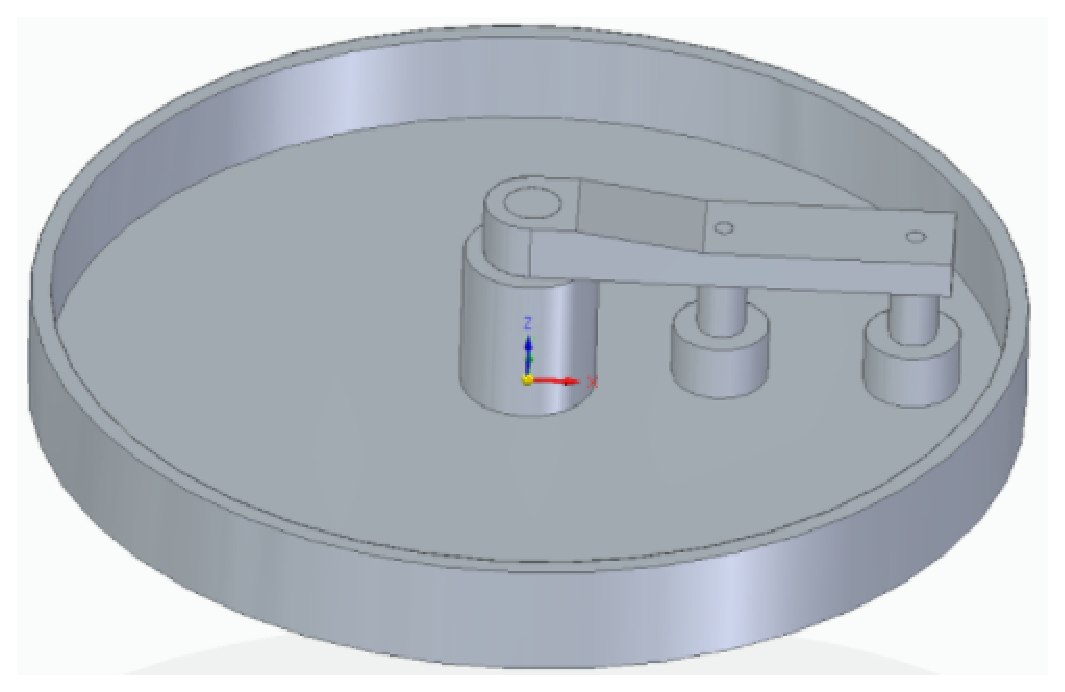
\includegraphics[height=3.1cm]{img/eps/swag.eps}
          \scalebox{0.8}{[3]たわみ量を少なくする設計}
        \end{center}
      \end{minipage}
    \end{tabular}
    \caption{設計した3種類のアームロボット}
    \label{3-arm}
  \end{center}
\end{figure}

図\label{3-arm}に示した3種類のロボットアームの断面形状において機構及び構造の解析を行い,表\ref{first-spec}の仕様を満たすように再設計を行う.
